\documentclass{scrreprt}
\usepackage[margin=0.7in,footskip=.5cm]{geometry} %réduire marges

\usepackage[frenchb]{babel} %en Français
\usepackage[utf8]{inputenc}
\usepackage[colorlinks=true,urlcolor=blue,linkcolor=blue]{hyperref}
\usepackage[T1]{fontenc}
\usepackage[babel=true]{csquotes}
\usepackage{array}
\usepackage{multicol}
\usepackage{hyperref}

\usepackage[pdftex]{graphicx}
\usepackage{epsfig}

\setlength{\parindent}{0cm}
\setlength{\parskip}{1ex plus 0.5ex minus 0.2ex}
\newcommand{\hsp}{\hspace{20pt}}
\newcommand{\HRule}{\rule{\linewidth}{0.5mm}}

\begin{document}
\pagenumbering{arabic}
\begin{titlepage}
  \begin{sffamily}
  \begin{center}

    % Upper part of the page. The '~' is needed because \\
    % only works if a paragraph has started.
    
\includegraphics[scale=0.2]{images/logo_upmc.png}~\\[1.5cm]

    \textsc{\LARGE PSAR}\\[2cm]

    \textsc{\Large Rapport}\\[1.5cm]

    % Title
    \HRule \\[0.4cm]
    { \huge \bfseries iBalezator\\[0.4cm] }

    \HRule \\[2cm]
    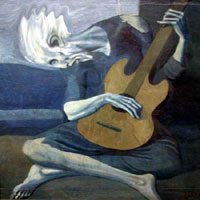
\includegraphics[scale=0.4]{images/picasso_le_vieux_balese.jpg}
    \\[2cm]


    % Author and supervisor
    \begin{minipage}{0.4\textwidth}
      \begin{flushleft} \large
        Adrien \textsc{Ferreira}\\
        Alexandra \textsc{Hospital}\\
      \end{flushleft}
    \end{minipage}
    \begin{minipage}{0.4\textwidth}
      \begin{flushright} \large
        \emph{Encadrant :} Fabrice \textsc{Kordon}\\
        \emph{Client : } Thomas \textsc{Baspeyras}
      \end{flushright}
    \end{minipage}

    \vfill

    % Bottom of the page
    {\large 4 mai 2015}

  \end{center}
  \end{sffamily}
\end{titlepage}

\tableofcontents \newpage

\setlength{\parindent}{1cm}
\chapter{Introduction}

\noindent Ce document constitue le rapport du projet iBalezator.\\
\noindent \textbf{Maitrise d'ouvrage :} Thomas \textsc{Baspeyras}, Fabrice \textsc{Kordon} \newline
\noindent \textbf{Maitrise d'oeuvre :} Adrien \textsc{Ferreira}, Alexandra \textsc{Hospital}\newline
\smallbreak

Le produit du projet étant directement lié à la musique, quelques notions importantes pour comprendre son intégralité ont été repertoriées en annexe.

\section{Sujet}

iBalezator est une application pour petit terminaux sous \textit{iOS} 8 (de 3,5 à 4,7 pouces) qui consiste en un jeu de devinette pour mémoriser la disposition des notes sur le manche d’une guitare. 
Elle s'inspire du site Internet Le Balezator \url{http://www.orbite.info/balezator/}, créé par Thomas \textsc{Baspeyras}.
\noindent L'application comporte deux modes de jeu : 
\begin{itemize}
\item Le mode manche/clavier, dans lequel l'utilisateur lit une question sur le manche et répond sur un clavier
\item Le mode portée/manche, dans lequel l'utilisateur lit une question sur la portée et répond sur le manche
\end{itemize}

L’application s’adresse à des guitaristes débutants connaissant le principe de jeu sur le manche d'une guitare et sachant lire une partition musicale. Elle propose une aide à la mémorisation des notes sur le manche de la guitare et à la lecture d’une partition.

\section{Problématique}

La problématique de ce projet est de pouvoir adapter un mode de jeu présent sur le site web Le Balezator -- le mode manche/clavier -- sur petits terminaux en restant ludique et ergonomique; ainsi que d'implémenter un nouveau mode de jeu -- le mode portée/manche.

\chapter{Présentation du produit}

\section{Fonctionnalités}

\subsection{Mode manche/clavier}


\begin{figure}[!ht]
	\centering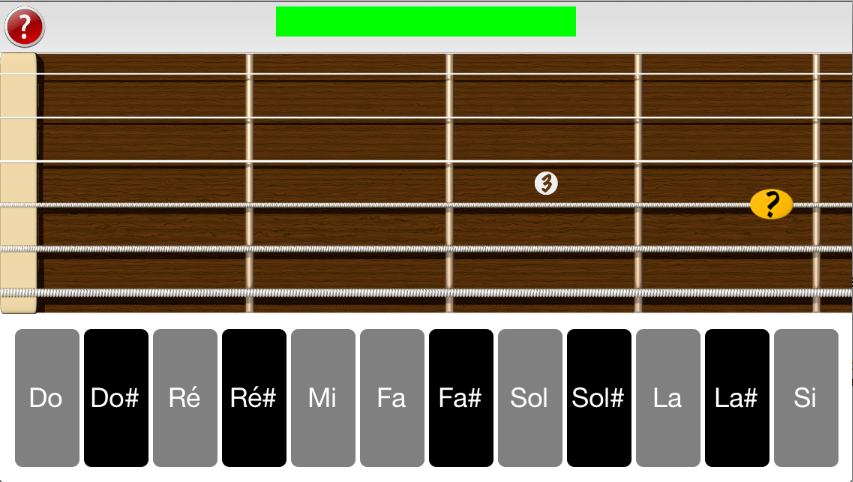
\includegraphics[width=7cm]{images/clavier_first_question.png}
     	\caption{Le mode manche/clavier}
\end{figure}


L'application démarre en mode manche/clavier.

\noindent Le mode est composé :
\begin{itemize}
	\item D'une barre d'outils comprenant une barre de score et une aide
	\item D'un manche de guitare qu'il est possible de faire glisser vers la gauche pour travailler sur les parties plus aiguës
	\item D'un clavier composé des 12 notes de la gamme : \textit{Do}, \textit{Do}\#, \textit{Ré}, \textit{Ré}\#, \textit{Mi}, \textit{Fa}, \textit{Fa}\#, \textit{Sol}, \textit{Sol}\#, \textit{La}, \textit{La}\#, \textit{Si}
\end{itemize}
\bigbreak
Une note est tirée aléatoirement et apparaît sous forme de question sur le manche de la guitare symbolisée par une pastille jaune (figure \ref{fig:fig1}) indiquant à l’utilisateur la note à trouver. Le son de la note en question est émis.
À l’aide du clavier présenté dans la partie basse de l’écran, l’utilisateur choisit sa réponse, la note qu’il pense lire.\\
\smallbreak
Si l'utilisateur saisit une mauvaise réponse, la fausse note apparaît sous forme de pastille rouge (figure \ref{fig:fig3}) avec le son correspondant à cette fausse note.
S'il y a plusieurs possibilités d'affichage de la mauvaise note sur le manche, l'application favorisera une position proche de la note à trouver.
L’application invite l'utilisateur à réessayer jusqu’à ce qu’il trouve la bonne réponse, avec le son de la note à trouver.
Par exemple, sur la figure ci-dessus, la note à trouver est un \textit{Fa}\#. 
Tant que l'utilisateur n'aura pas répondu la touche \textit{Fa}\# du clavier, l'application reposera cette même question.\\
Si l’utilisateur saisit une bonne réponse, la pastille sur le manche s’allumera en vert (figure \ref{fig:fig2}) pendant une seconde, le son de la bonne note sera émis, et l’application passera à la question suivante.\\
L'utilisateur a la possibilité de faire défiler le manche pour choisir la partie sur laquelle il souhaite travailler. 
Les questions posées concerneront toujours la partie du manche visible à l'écran.

\begin{figure}[!ht]
   \centering
   \begin{minipage}[t]{5.5cm}
      \centering
      
\includegraphics[width=1.5cm]{images/fingering_question.png}
      \caption{Question}
	\label{fig:fig1}
   \end{minipage}
   \begin{minipage}[t]{5.5cm}
      \centering
      
\includegraphics[width=1.5cm]{images/fingering_good.png}
      \caption{Bonne réponse}
	\label{fig:fig2}
   \end{minipage}
   \begin{minipage}[t]{5.5cm}
      \centering
      
\includegraphics[width=1.5cm]{images/fingering_bad.png}
      \caption{Mauvaise réponse}
	\label{fig:fig3}
   \end{minipage}
\end{figure}

\newpage

\subsection{Mode portée/manche}

\begin{center}
\begin{figure}[!ht]
     \centering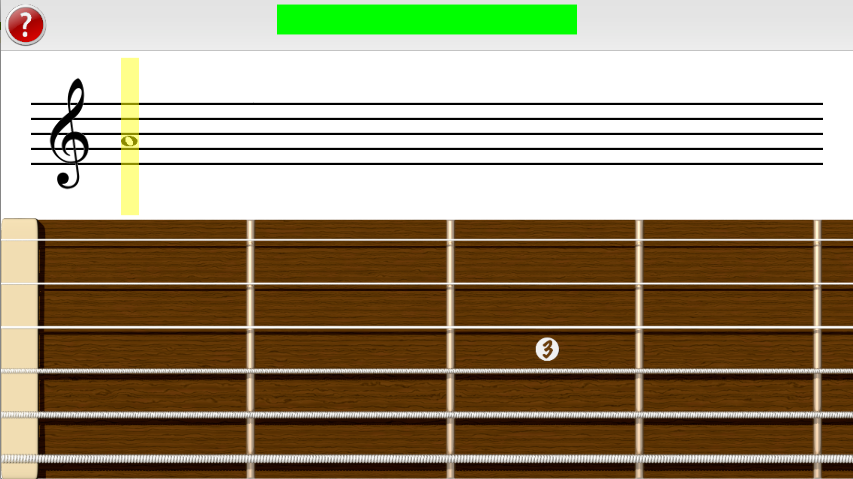
\includegraphics[width=7cm]{images/portee_first_question.png}
	\label{fig:p_m}
      \caption{Le mode portée/manche}
\end{figure}
\end{center}

\noindent Le mode portée/manche est composé :
\begin{itemize}
	\item D'une barre d'outils comprenant une barre de score et une aide
	\item D'une portée en clé de sol
	\item D'un manche de guitare qu'il est possible de faire glisser vers la gauche pour travailler sur les parties plus aiguës
\end{itemize}

\bigbreak

L'ensemble de notes à afficher est tiré aléatoirement. La première note à trouver est affichée sous forme de question symbolisée par une surbrillance jaune (figure \ref{fig:p_m}).
Le son de la note à trouver est émis.
L'utilisateur lit les notes qui apparaissent sur la portée.
À l'aide du manche de guitare dans la partie basse de l'écran, l'utilisateur choisit sa réponse en tapant sur la position souhaitée.\\

Si l'utilisateur saisit une mauvaise réponse, la surbrillance de la note deviendra rouge et la note qu'il a effectivement touchée sur le manche apparaîta sur la partition (figure \ref{fig:pm_mauvaise}), avec le son correspondant à cette fausse note. L'utilisateur est invité à réessayer jusqu'à ce qu'il trouve la bonne réponse.
La barre de score est mise à jour.\\
Si l’utilisateur saisit une bonne réponse, la surbrillance devient verte (figure \ref{fig:pm_bonne}) pendant une seconde, le son correspondant à cette bonne réponse est émis  et l’application passe à la question suivante : la note apparaît sur la portée en subrillance jaune.
\\
L'utilisateur a la possibilité de faire défiler le manche pour choisir la partie qu'il souhaite travailler. Les questions posées concerneront toujours la partie du manche visible à l'écran.
\bigbreak
\begin{figure}[!ht]
   \centering
   \begin{minipage}[t]{8cm}
      \centering
      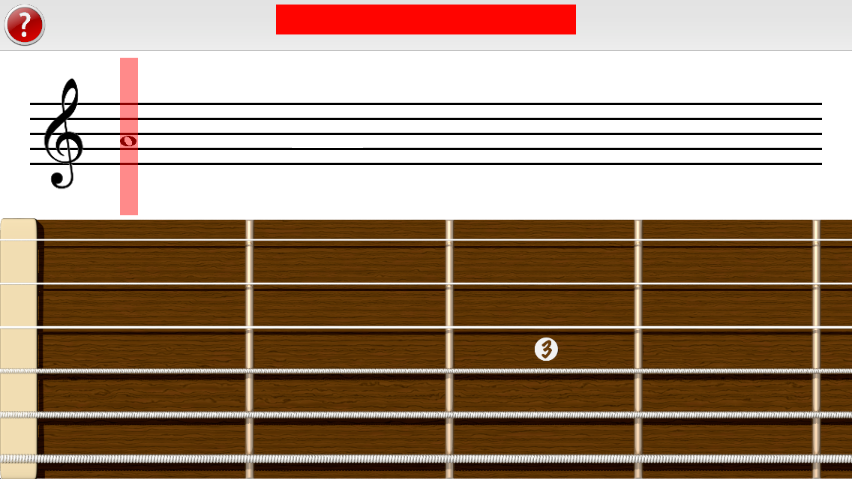
\includegraphics[width=7cm]{images/portee_first_bad_question.png}
      \caption{Mauvaise réponse}
	\label{fig:pm_mauvaise}
   \end{minipage}
   \begin{minipage}[t]{8cm}
      \centering
      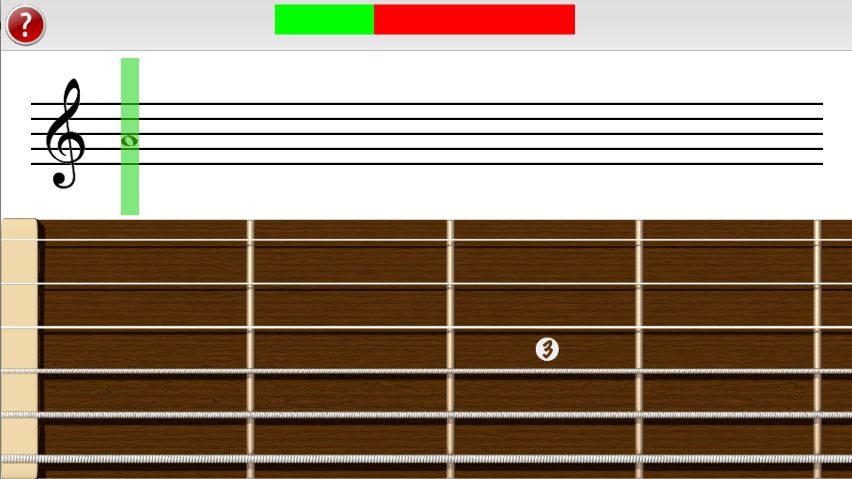
\includegraphics[width=7cm]{images/portee_first_good_question.png}
      \caption{Bonne réponse}
	\label{fig:pm_bonne}
   \end{minipage}
\end{figure}


% 8va
%%%%%%%%%% Image à rajouter pour l'octava
La particularité de la portée est que quand les notes sont hautes (pour notre application : à partir du \textit{Mi} 3 lignes au dessus de la portée, inclus), on utilise en solfège une notation \texttt{8va} (octava) qui permet d'écrire les notes une octave plus bas que leur place réelle (cf : paragraphe \ref{octava} pour plus de détails techniques). 
Ainsi, on évite d'ajouter des lignes au dessus de la portée, ce qui rendrait peu claire la lecture.
L'application prend en compte cette notation pour les notes qui sont plus aiguës que le \textit{Ré}\#, 2 lignes au dessus de la portée. À partir du \textit{Mi} suivant, les notes sont écrites une octave en dessous.\\

\subsection{Score et aide}


Une barre de score commune aux deux modes est présente dans la barre d'outils, dans la partie supérieure de l'écran. 
Elle fait état de la progression de l’utilisateur en affichant une jauge en proportion de bonnes réponses (en vert) et de mauvaises réponses (en rouge).\\
Une vue d'aide a été prévue sur l'application. Aujourd'hui, elle n'est pas complétée.


\section{Manuel d'utilisation}


L'application démarre en mode manche/clavier.
Pour changer de mode, il faut effectuer un glissé vertical sur l'écran.

\subsection{Mode manche/clavier}

\begin{figure}[!ht]
  \begin{minipage}{6cm}
      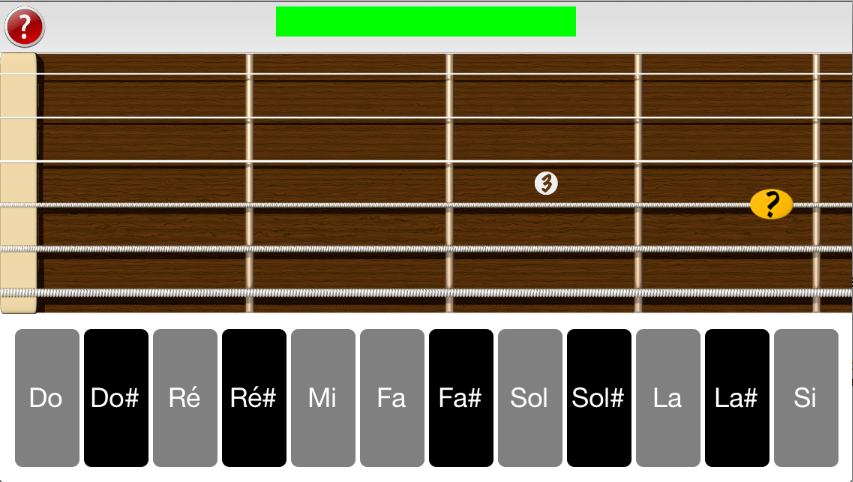
\includegraphics[width=5cm]{images/clavier_first_question.png}
  \end{minipage}\hfill
  \begin{minipage}{10cm}
  {Au démarrage de l'application, le système commence en mode manche/clavier. Une question est posée, représentée par un marqueur jaune. Le son de la note à trouver est joué.
	 Pour répondre, appuyer sur une des touches du clavier.}
   \end{minipage}
\end{figure}


\begin{figure}[!ht]
  \begin{minipage}{6cm}
      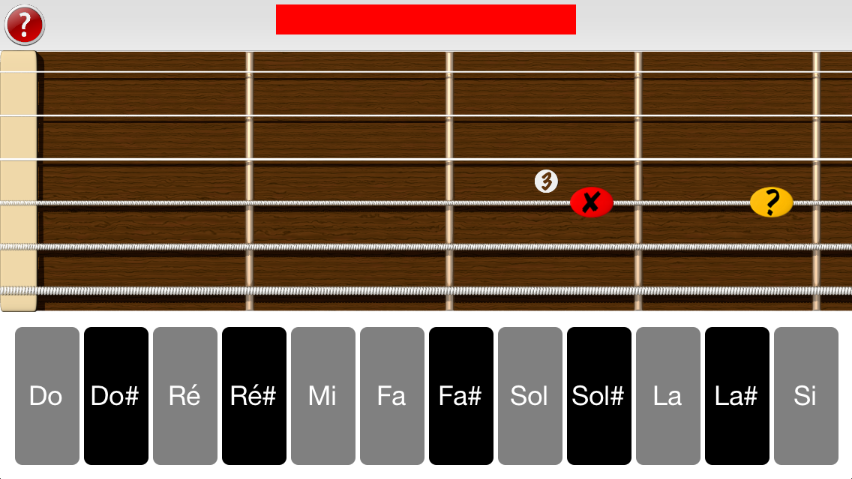
\includegraphics[width=5cm]{images/clavier_first_bad_question_2.png}
  \end{minipage}\hfill
  \begin{minipage}{10cm}
  {Si la réponse est mauvaise, le marqueur le notifie (marqueur rouge). Le son de la fausse note est joué. Répondre de nouveau jusqu'à ce que la réponse soit acceptée.}
   \end{minipage}
\end{figure}


\begin{figure}[!ht]
  \begin{minipage}{6cm}
      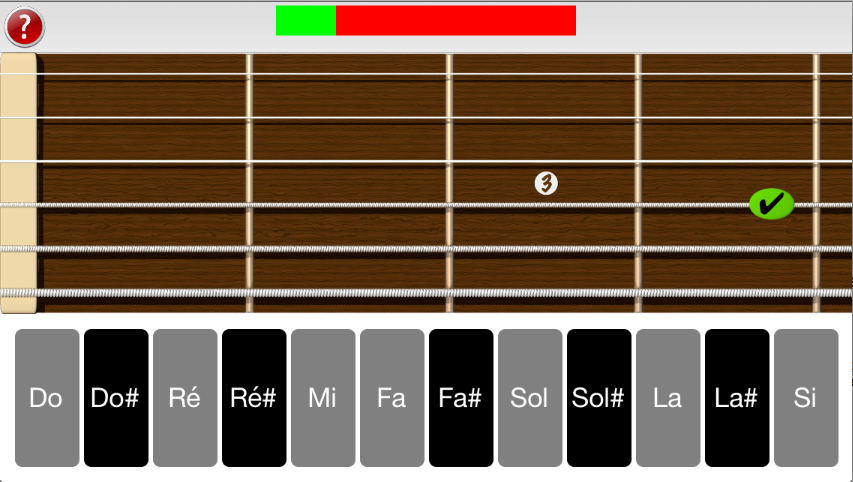
\includegraphics[width=5cm]{images/clavier_first_good_question.png}
  \end{minipage}\hfill
  \begin{minipage}{10cm}
  {Si la réponse est bonne, le marqueur le notifie (marqueur vert), le son de la note est joué, puis une nouvelle question est posée. Répondre comme précédemment.}
   \end{minipage}
\end{figure}

\bigbreak
\textit{N.B : Si le manche est changé de place, une nouvelle question sera générée. Les questions concernent toujours la partie visible du manche. Répondre comme expliqué précedemment.}
\newpage

\subsection{Mode portée/manche}

Pour changer de mode, il faut effectuer un glissé vertical sur le manche.


\begin{figure}[!ht]
  \begin{minipage}{6cm}
      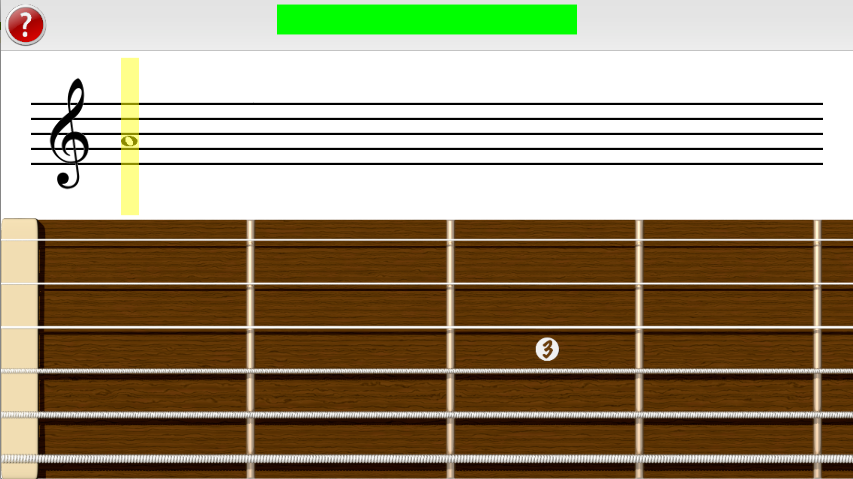
\includegraphics[width=5cm]{images/portee_first_question.png}
  \end{minipage}\hfill
  \begin{minipage}{10cm}
  {Après avoir changé de mode, une question est posée sur la portée : la note apparaît surlignée en jaune. Le son de la note à trouver est joué. Pour répondre, appuyer sur une position sur le manche.}
   \end{minipage}
\end{figure}


\begin{figure}[!ht]
  \begin{minipage}{6cm}
      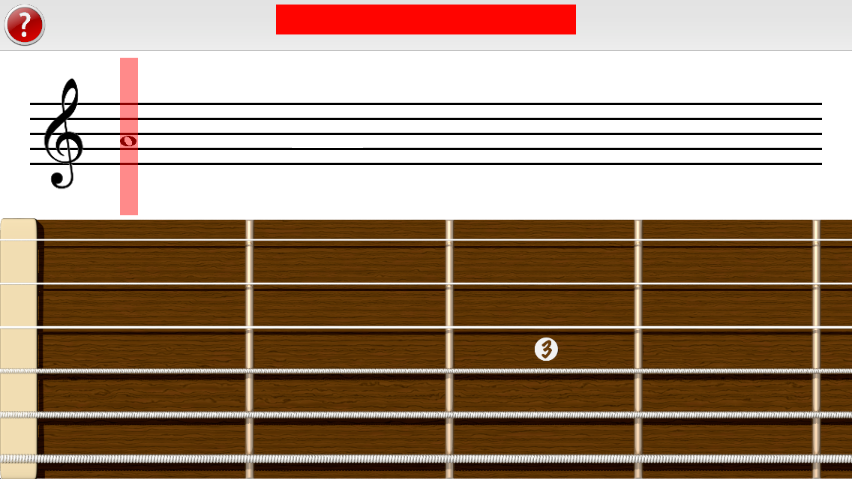
\includegraphics[width=5cm]{images/portee_first_bad_question.png}

  \end{minipage}\hfill
  \begin{minipage}{10cm}
  {Si la réponse est mauvaise, la surbrillance le notifie (rouge). La fausse note apparaît sur la portée et le son correspondant à cette fausse note est joué. Répondre de nouveau jusqu'à ce que la réponse soit acceptée.}
   \end{minipage}
\end{figure}


\begin{figure}[!ht]
  \begin{minipage}{6cm}
      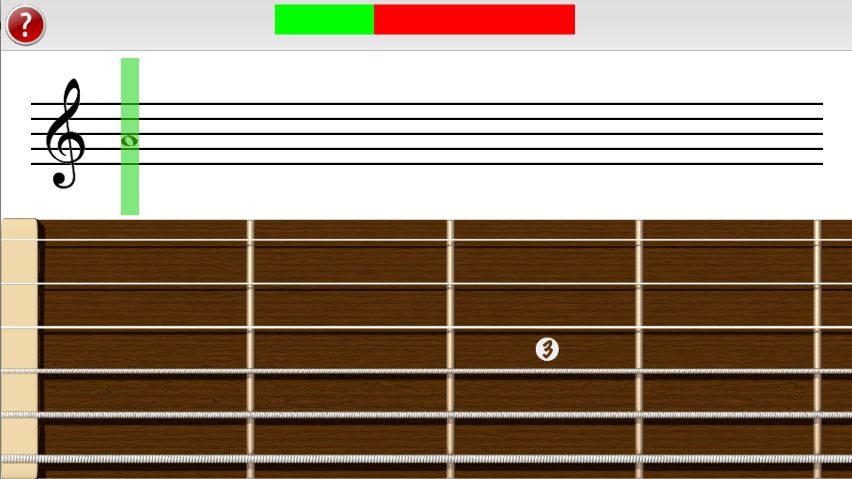
\includegraphics[width=5cm]{images/portee_first_good_question.png}
  \end{minipage}\hfill
  \begin{minipage}{10cm}
  {Si la réponse est bonne, la surbrillance le notifie (vert) pendant une seconde, le son de la note est joué, puis une nouvelle question est posée.}
   \end{minipage}
\end{figure}


\begin{figure}[!ht]
  \begin{minipage}{6cm}
      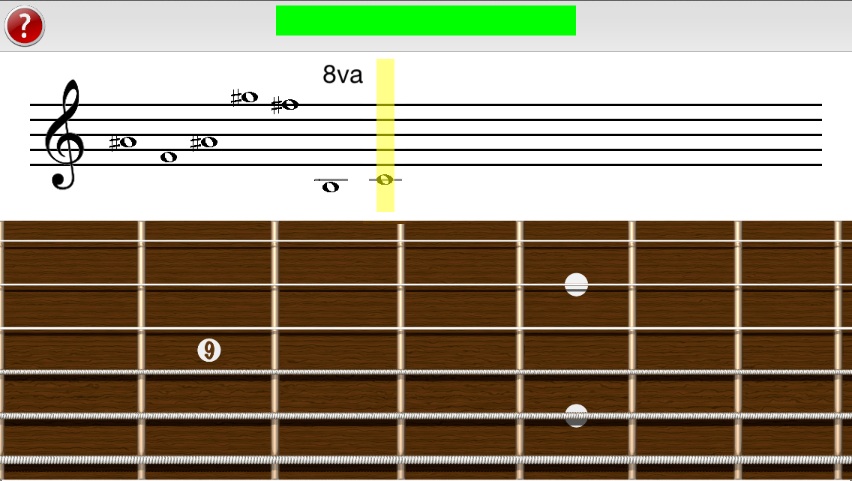
\includegraphics[width=5cm]{images/portee_octava.png}
  \end{minipage}\hfill
  \begin{minipage}{10cm}
  {Dans le cas où le manche a été déplacé et que la frette 12 apparaît à l'écran, il est possible d'avoir la notation \texttt{8va} affichée. À partir de cette notation, lire les notes une octave au dessus.}
   \end{minipage}
\end{figure}
% Un peu similaire au paragraphe suivant, on peut
% peut-être tout mettre dans un seul :
% \section{Comparaison avec le cahier des charges}


\section{Recettes : bilan des tests de validation}

Une série de tests a été réalisée sur l'application par l'équipe de développement, en jouant au jeu de l'iBalezator.\\
\smallbreak

Les interfaces graphiques de chacun des modes ont été réalisées d'après les maquettes fournies par notre client, Thomas \textsc{Baspeyras}. Chaque élément du jeu (manche, clavier, portée, barre de score) correspond à un pourcentage de la zone de l'écran. 
Les touches du clavier sont disposées en lignes et colorées à la façon d'un piano (c'est-à-dire que les notes dièses sont plus foncées que les notes \enquote{normales}) et dimensionnées de façon à ce que l'utilisateur ait un touché confortable sur ces touches. \\
De même, le manche de guitare doit être assez grand pour que le touché sur une position soit précis. Il doit y avoir au moins 4 cases à l'écran du côté sillet du manche, même sur un petit écran (i.e : 3,5 pouces).
\newpage
\subsection{Mode manche/clavier}

L'application est capable de créer un jeu et de garder un enchaînement logique des événements.
Le système tire au sort une note dans la partie visible du manche, affiche le marqueur de question, joue la note puis attend la réponse de l'utilisateur. Cela signifie que l'application est capable de mettre en relation une note avec sa position sur le manche, et le son lui correspondant.\\
Le système est capable de détecter une réponse entrée par l'utilisateursur le clavier, de l'analyser et de la qualifier de bonne ou mauvaise réponse. Il le notifie au moyen de l'affichage du marqueur vert ou rouge, il joue le son correspondant à la note entrée par l'utilisateur. \\
Si l'on change de position sur le manche, une nouvelle question est générée, toujours dans la partie visible du manche.\\
La mise à jour du score est également gérée.\\
\medbreak
Bilan : le mode manche/clavier est conforme aux besoins détaillés dans le cahier des charges.


\subsection{Mode portée/manche}


L'application est capable de créer un jeu et de garder un enchaînement logique des événements.

Le système tire au sort une note dans la partie visible du manche, la dessine sur la portée, puis attend la réponse de l'utilisateur. 
L'application est capable de mettre en relation une note et sa représentation graphique sur la portée, notamment lorsque cette note est \enquote{diésée} ou non. Les notes \textit{Mi} et \textit{Si} ne seront jamais affichées avec un dièse.\\
Le système est capable de détecter une réponse entrée par l'utilisateur sur le manche, de l'analyser et de la qualifier de bonne ou mauvaise réponse. Il le notifie au moyen de l'affichage de la fausse note sur la portée, du surlignage rouge de la note et du son de la fausse note joué au moment du tap de l'utilisateur. Si l'on change de position sur le manche, une nouvelle question est générée, toujours dans la partie visible du manche.\\
Dans le cas où les notes sont trop aiguës pour être affichées sur la portée ou sur les 2 lignes au dessus de la portée, l'application est capable d'afficher un \texttt{8va} à partir duquel toutes les notes seront écrites une octave en dessous de leur position réelle.\\

Lorsque la portée est remplie et que la dernière note a été validée comme bonne réponse, la portée est complètement vidée pour laisser place à un nouvel ensemble de notes tirées aléatoirement, comme au lancement de ce mode.
\medbreak
Bilan : le mode portée/manche est conforme aux besoins détaillés dans le cahier des charges.

\subsection{Changement de mode}

Le changement de mode s'effectue par un glissé vertical sur l'écran. 

\chapter{Réalisation et implémentation}
\section{Particularité du solfège}
\label{portee}
\begin{figure}[!ht]
  \begin{minipage}{11cm}
      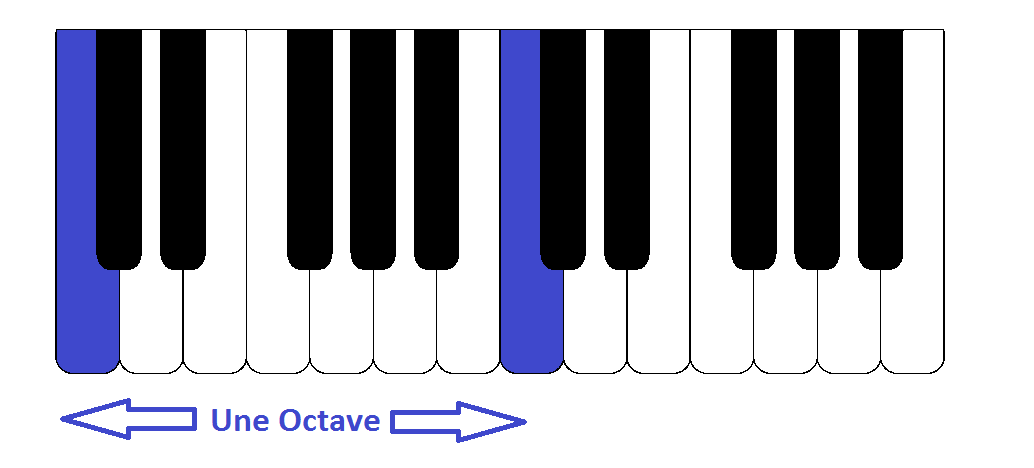
\includegraphics[width=10cm]{images/implementation/clavier-piano-octave.png}
  \end{minipage}\hfill
  \begin{minipage}{7cm}
  {En musique occidentale, une octave est divisée en 12 demi-tons. }
   \end{minipage}
\end{figure}

\begin{figure}[!ht]
  \begin{minipage}{11cm}
      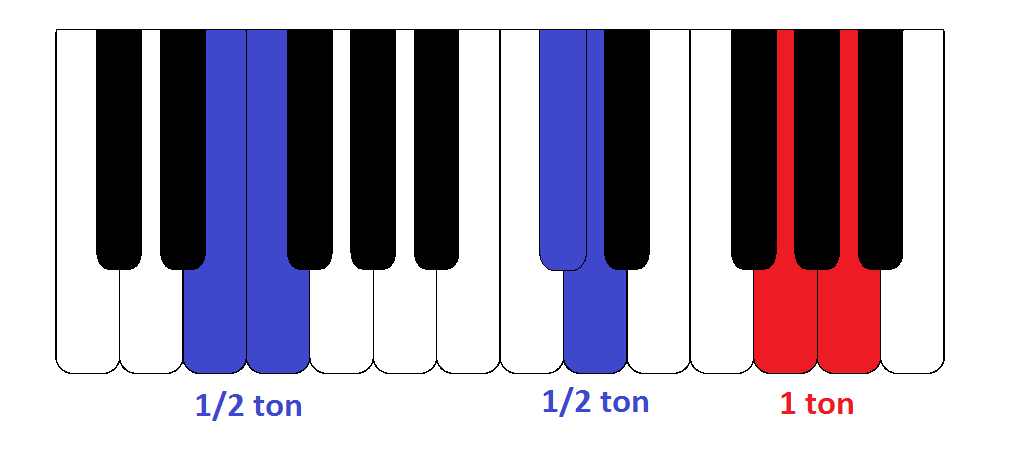
\includegraphics[width=10cm]{images/implementation/clavier-piano-demi-ton-ton.png}
  \end{minipage}\hfill
  \begin{minipage}{7cm}
  {Sur un piano, un demi-ton est matérialisé par deux touches adjacentes. Une gamme est composée de tons et demi-tons.}
   \end{minipage}
\end{figure}

La gamme majeure est composée de 2 tons puis un demi-ton puis trois tons et un demi-ton.
Si l'on part d'un \textit{Do} et que l'on suit un tel schéma, sur un piano, cela correspond aux touches blanches.
Une octave est divisée selon la structure d'une gamme majeure.
Chaque touche blanche correspond à un degré de la gamme.
Deux degrés sont donc séparés soit par un ton soit par un demi-ton.
Un intervalle est le nombre de demi-tons qui sépare deux degrés.
La tessiture d'un instrument c'est la totalité des notes qu'il est capable de jouer.
Dans le cadre de ce projet, cette particularité de la théorie musicale apporte sont lot de problématiques notamment pour le placement des notes sur une portée, le calcul d'intervalle, la structure de l'accordage de la guitare.
\newline
Nous avons mis au point un algorithme qui permet de consommer successivement et hétérogénéiquement des demi-tons et résoudre les problèmes cités ci-dessus.
La structure interne d'une octave est irégulière mais elle est cyclique.
Cette cyclicité nous a permis d'utiliser les modulos sur les indices pour nous déplacer sur toute la tessiture de la guitare avec une seule structure de données.

Dans l'algorithme ci-dessous, la gestion des dièses est omise, elle consiste presque exclusivement à vérifier à la fin de la boucle que \texttt{resteDemiTons} est égal à zéro.
Partant de la note la plus grave que la guitare peut jouer (paramètre \texttt{a}), on peut ainsi savoir où placer \texttt{b} sur la portée.
Ceci en multipliant un décalage fixe par rapport aux coordonnées constantes connues de \texttt{a} sur la portée.

\newpage
\begin{figure}[h!]
\vspace*{\fill} 
\begin{center}
  \begin{verbatim}
  /*
  * Fonction permettant de trouver le nombre d'interlignes entre deux notes sur la portée.
  * Retourne le nombre d'interlignes séparant a et b
  * a doit être plus grave que b.
  * a : Note de départ
  * b : Note d'arrivée
  */
  Fonction nombreDeDemiTonsEntreAB(a : Note, b : Note ) : Entier
  DébutFonction
    // deux tons, un demi-ton, trois tons, un demi-ton
    Constante tonaliteMajeure = [2, 2, 1, 2, 2, 2, 1];
    
    Variable resteDemiTons : Entier; //restant à consommer
    Variable nbInt : Entier; // Nombre d'interlignes
    Valiable cmpt : Entier; // itérateur sur tonaliteMajeure

    resteDemiTons = a.nbDemiTonsAvec(b);
    cmpt = 0;
    nbInt = 0;

    TantQue resteDemiTons > 0 
    Faire
      //consomation des demi-tons en fonction de la structure de la gamme
      resteDemiTons = resteDemiTons - tonaliteMajeure[cmpt modulo tonaliteMajeure.taille ];
      cmpt++;
      nbInt++;
    FinTantQue

    retourner nbInt;
  FinFonction
  \end{verbatim}
    \caption{Algorithme de calcul de nombre d'interlignes entre deux notes}
\end{center}
\vspace*{\fill}
\end{figure}
\newpage

% expliquer l'algorithme le dérouler.
%%% Accordage de la guitare
%%% Structure d'une gamme
%%% Portée, un degré, différent pas 

\newpage
\section{Mise en relation d'une note sur le manche avec une note sur la portée}
% octava, tout faire rentrer, biaiser l'aléatoire,
\label{octava}
Une des directives du cahier des charges est d'afficher le symbole \texttt{8va} quand une note est très aiguë.
Ce symbole indique à l'utilisateur qu'il doit lire la note affichée une octave plus aiguë que ce qui est affiché sur la portée. 
Une autre directive du cahier des charges est qu'une fois qu'une note est octaviée, celles qui suivent doivent l'être également.
Ceci dit, certaines notes ne peuvent pas être lues en notation octaviée (car elles n'existent pas sur la guitare). 
Sur une même position visible du manche, on aura donc des notes qui peuvent être octaviées et d'autres non.
Or, nous utilisons un tirage aléatoire pour choisir les notes à afficher.
Voilà pourquoi nous avons dû biaiser l'aléatoire.
Nous tirons des notes aléatoire et si une apparait comme nécessitant d'être octaviée, nous déterminons un sous ensemble de notes qui peuvent être octaviées parmi toutes celles sur la partie visisble du manche.
Puis nous relançons l'aléatoire sur ce nouveau sous-ensemble. 
\newline

% notes enharmoniques
Sur un manche de guitare, il est possible de jouer une même note/fréquence à différents endroits du manche (appelées notes enharmoniques).
Ces diférentes notes peuvent être sur une même partie visible du manche.
Nous avons dû traîter cette particularité dans nos algorithmes.
Par exemple, en mode manche/clavier, quand une note est affichée et que l'utilisateur saisit une mauvaise réponse au clavier, il est impossible de savoir quelle note il avait en tête.
Voilà pourquoi nous avons utilisé un algorithme qui à une note donnée sur le manche trouve la note erronée la plus proche.
Ce même phénomène survient en mode portée/manche.
Quand l'utilisateur lit une note sur la portée il a potentiellement plusieurs positions sur lesquelles il peut la jouer.
Dans ce cas là, il faut donc trouver et accepter toutes les réponses valides possibles.
%TODO schéma
\newline

%calcul des lignes supplémentaires
Comme nous l'avons vu dans la section \ref{portee} le positionnement d'une note sur la portée dépend d'une structure hétérogène.
Or, nous avons décidé de dessiner la portée grâce aux fonctionnalités d'\textit{iOS}.
Des lignes supplémentaires sont ajoutées en haut (respectivement en bas) de la portée quand une note est trop aiguë (respectivement grave) pour rentrer sur les cinq lignes de base.
Mais, ces lignes suplémentaires ne sont à dessiner que sous les notes concernées.
Voilà pourquoi, en conjonction de l'algorithme présenté en section \ref{portee}, nous avons dû déterminer la quantité de lignes supplémentaires à ajouter pour chaque note du tirage.
Ceci au moment de l'afffichage de chaque note, individuellement.

\subsection{Mise en relation de coordonnées d'image de manche avec une Note}
% obtenir la partie visible du manche 
Le tirage des notes/questions auxquelles l'utilisateur est invité répondre doit toujours être en fonction de la partie du manche affichée à l'écran. 
Seules les frettes affichées dans leur totalité sont éligibles à l'aléatoire.
Le manche de la guitare étant simplement une image que l'on peut faire défiler horizontalement, il a donc fallu convertir de simples coordonnées en frettes.
\textit{iOS} nous donne accès à l'offset de l'image et les dimensions de l'écran.
Suite à cela nous avons stocké les coordonnées des frettes et déterminé lesquelles étaient affichées dans leur totalité.
\newline

% convertir une position en note et convertir une note en position
Nous avons aussi stocké les coordonnées des cordes.
De ce fait nous avons pu opérer à des croisements car quand l'utilisateur tape sur l'image du manche, \textit{iOS} nous donne les coordonnées correspondantes.
À un tape sur l'écran, il est donc possible de retrouver la note que l'utilisateur a voulu sélectionner.
\newpage

\section{Son}
% ne pas stocker tous les fichiers audio
Les notes affichées à l'écran doivent aussi être jouées sur les hauts-parleurs/écouteurs du terminal.
Le client avait clairement demandé dès le départ qu'il ne voulait pas que l'on stocke les 36 fichiers audio correspondant aux notes qu'il est possible de jouer.
En fonction de la qualité des enregistrements, ces fichiers peuvent être volumineux et augmenter le poids de l'application et nuire à son succès.
\newline

AudioKit est une bibliothèque de génération de fréquences sonores pour \textit{iOS}.
Elle est écrite en \textit{Objective-C} mais il est possible de lancer des fonctions écrites dans ce langage depuis \textit{Swift} grâce à une interface.
Cette bibliothèque est intéressante car elle permet de jouer des notes avec des simulations d'intruments.
En jouant sur les caractéristiques de vie du son elle va générer des fréquences qui ressemblent à une guitare, une mandoline, un vibraphone, entre autres.
Nous avons créé un controleur capable de prendre en paramètre des objets Note de notre modèle et ainsi masquer les complexités de la bibliothèque dans l'implémentation de la logique du jeu.
Cette bibliothèque n'utilise aucun fichier audio et est très légère.
\newline

% jeunesse de la bibliothéque, peu de documentation
Cependant elle est relativement jeune et il est difficile de trouver des articles, des exemples, de l'aide.
L'installation de la bibliothèque a été un problème pendant une longue période du développement.
Par la suite, un tutoriel vidéo expliquant comment installer et compiler la bibliothèque a été publiée sur le site officiel, ce qui nous a permis de l'intégrer au projet.
Il apparaît qu'elle n'est pas Thread-safe ce qui a posé des problèmes avec l'utilisation de Timers et aucun documentation sur ce point n'est disponible.
Il n'y a également aucune documentation sur la manière de compiler et exporter une application stand-alone qui embarque cette bibliothèque.

% calcul de fréquence
Le client a émis le souhait d'avoir une prise en charge de la norme de MIDI des classification des notes.
Ainsi, chaque note se voit attribuer une fréquence normalisée en fonction de la formule mathématique suivante. 
\[f_{n} = f_{0} \times 2^{\frac{n}{12}}\]

Où $f_{0}$ est, par exemple, la fréquence standard du \textit{La} 440 Hz et $n$ le nombre de demi-tons au dessus de cette même note.
\newline

\section{Temporisation}
% rappel du cahier des charges
Une des demandes du cahier des charges était de temporiser l'enchaînement des questions.
Ainsi, si l'utilisateur saisit une réponse valide, on affiche un indicateur, on attend une seconde puis on passe à la question suivante.
Pendant ce lapse de temps, il est important de désactiver certaines fonctionnalités de l'interface.
Par exemple, en mode clavier/manche, si l'utilisateur sélectionne d'autres notes sur le clavier pendant la temporisation, ces réponses doivent être ignorées.
Le fonctionnement par défaut d'\textit{iOS} est de tous les traiter après la fin du timer. 
Nous avons donc dû gérer les désactivations de fonctionnalités en fonction du contexte.

\section{Architecture finale}%changer de nom

L'architecture finale de l'application est restée, dans sa majeure partie, fidèle au diagramme de classe élaboré en phase d'analyse.
\newline

Quelques madifications ont cependant été apportées.
Le modèle, tout d'abord, compte une classe de plus : \texttt{MainModel}.
Cette classe a été créée pour stocker les données communes aux deux modes de jeu.
Nous pensions au début que chaque mode de jeu tiendrait à jour son propre score.
Après concertation avec le client, ce dernier à jugé plus pertinent que le score soit commun aux deux modes de jeu.
Le mode de jeu courant a été également stocké dans cette classe plutôt que dans le contrôleur principal.
Elle possède également en attribut deux instances correspondant aux deux modèles des deux modes de jeu.
\newline

L'affichage d'une fenêtre d'aide n'avait pas été spécifié dans le cahier des charges.
Cependant, comme son ajout été simple et rapide, nous l'avons ajouté.
Les classes \texttt{HelpController} et \texttt{HelpView} permettent la gestion d'un tel affichage.
La classe \texttt{HelpController} n'est présente que par souci de cohérence mais elle ne fait que relayer les ordres du \texttt{GameController}.
\newline

Les vues de l'application, conformément au patron MVC, ne s'occupent que des affichages sans traitements.
La vue \texttt{StaffView} embarque ceci dit une méthode privée qui calcule et affiche les lignes supplémentaires nécessaires au placement de la note.
Nous avons placé ce traitement dans la vue car c'est la vue qui connaît les dimensions de la portée et si la note à afficher est à l'intérieur des cinq lignes de base.
Le \texttt{StaffController} demande d'afficher la note à la vue à telle position et telle place les lignes supplémentaires si besoin.
Contrairement aux dièses, \texttt{8va} et marqueurs de réponse, les lignes supplémentaires n'ont pas de logique métier, elle sont simplement une aide à la lecture pour l'utilisateur.
\newline

La fonction \texttt{noteToFrequency()} aurait pu être placée dans la classe Note.
Cependant, nous l'avons laissée dans la classe \texttt{SoundController} dans le but d'isoler tous les aspects sonores dans cette classe.
\newline

\begin{figure}[!ht]
  \centering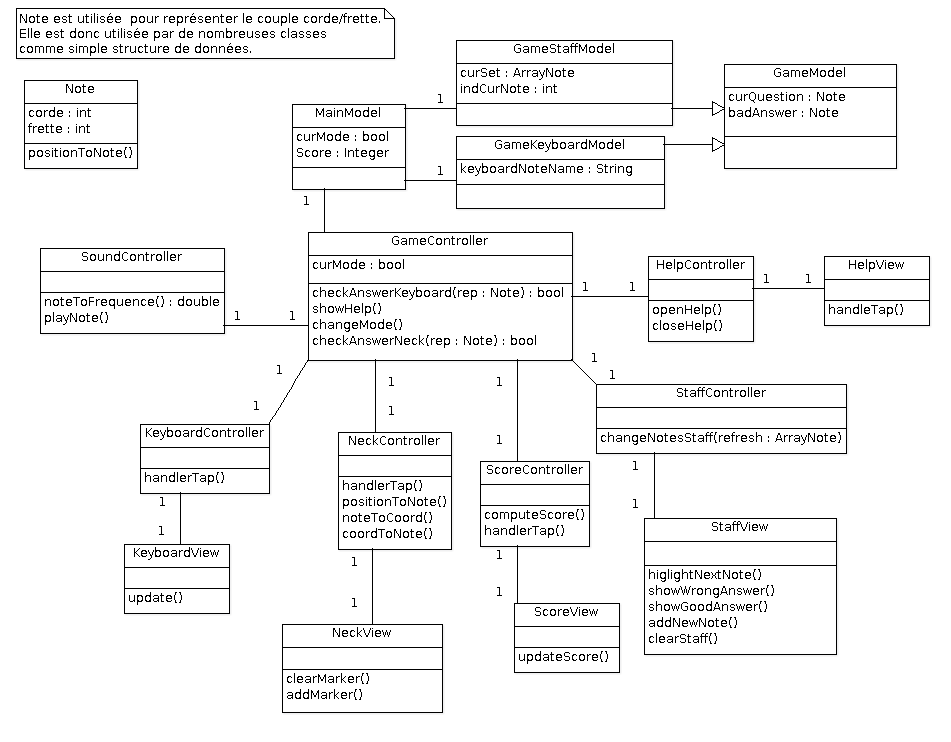
\includegraphics[width=\textwidth]{images/Diagrammedeclasses.png}
      \caption{Diagramme de classe de l'architecture finale}
\end{figure}

% TODO archtecure diagramme de classe final
% chaque vue à son MVC
% instanciation, liaison de l'architecture en Swift, pauvreté documentation
% événements, note clivage, relire cahier des charges
% pourquoi diviser le modèle ainsi, parler de tous les deltas avec le diagramme original
% décidé un score unique pour tous les modes

\section{Adaptation de l'application aux différentes tailles d'écran des terminaux}
% toujours afficher au moins 4 frettes sur la portée
Une des directives du cahier des charges était que l'on puisse toujours voir quatres frettes du manche, même en haut du manche, près du sillet.
Le client nous a fourni une image de manche qu'il voulait sur l'application.
Au vu des proportions de l'image, il n'était pas possible de faire apparaître quatre frettes.
En accord avec le client, nous avons donc décidé de tasser l'image et donc perdre les proportions de l'image originale.
Cette atypicité n'a pas posé de problème majeur, il a suffi de changer le tableau de coordonnées des frettes et codres.
\newline 

% dessiner plutôt qu'utiliser des images, adaptation à la taille de l'écran
L'affichage de la portée doit s'adapter à la taille de l'écran du terminal.
Une première approche consiste à stocker les images des 36 notes possibles dessinées sur une portée et les afficher côte-à-côte en fonction du tirage.
Cette méthode présente l'inconvénient de nécéssiter le stockage d'un grand nombre d'images, nous avons donc écarté cette solution.
Une deuxième méthode consiste à n'avoir qu'une image de portée et ensuite dessiner les notes sur ce fond. 
Plutôt que d'utiliser cette technique qui pourrait éventuelement faire apparaître la portée comme tassée en fonction de sa définition originale et les dimensions du terminal, nous avons décidé de dessiner la portée.
Les avantages de cette méthode est que l'on ne stocke aucune image, l'application sera donc d'autant plus légère.
De plus, le dessin étant vectoriel, c'est l'assurance d'avoir des traits nets quelque soit l'écran.
Enfin, il devient possible d'adapter l'écartement, la position et la hauteur des traits de la portée en fonction des capacités d'affichage du terminal.
Nous devons donc calculer le nombre et la position des lignes supplémentaires au besoin comme indiqué dans la section \ref{portee}.
\newline

% faire rentrer toute la tessiture de la guitare ?
La tessiture est l'ensemble des notes qui peuvent être jouées par un instrument donné.
La guitare est capable de jouer 36 notes différentes qui doivent toutes pouvoir être affichées sur la portée.
La portée doit donc avoir une taille conséquente pour pouvoir toutes les accueillir.
Les écrans pour lesquels nous devons développer étant petits, nous avons dû trouver la taille optimale pour la lecture sur la portée et utiliser le symbole \texttt{8va} en conséquence.
Ainsi, nous avons trouvé que le seuil optimal avant l'affichage du symbole \texttt{8va} est \textit{Ré}3 (deux lignes au dessus de la portée).
Ceci a pour effet d'abaisser la portée vers le bas et de faciliter la lecture des notes en tête de manche qui correspond certainement à la position la plus fréquente chez les guitaristes débutants.
\begin{figure}[!ht]
  \centering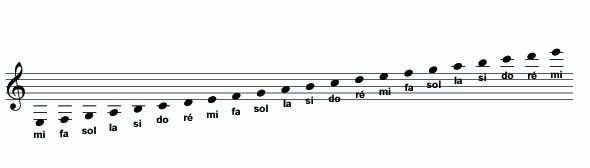
\includegraphics[width=\textwidth]{images/note_portee.jpg}
  \caption{Ensemble des notes que la guitare peut jouer (sa tessiture)}
\end{figure}
\newline

\chapter{Organisation}
\section{Équipe de développement, environnement de développement}
L'équipe de développement est composée d'Adrien Ferreira et d'Alexandra Hospital. 

Le matériel utilisé est un Mac mini sous MacOS 10.9.5. 
Les tests sont effectués sur un iPod touch MD720NF/A sous \textit{iOS} 8.1.3. Le déploiement sera fait du Mac vers l'iPod via le logiciel Xcode.

Le développement est effectué sur la plate-forme de développement Xcode 6.1 en langage \textit{Swift}.
Nous utilisons les différentes bibliothèques incluses par défaut pour le Swift. \\
La bibliothèque de son utilisée est audiokit (\url{http://audiokit.io/features/}) implémentée en \textit{Objective-C}.

\section{Organisation dans le temps}


\begin{figure}[!ht]
      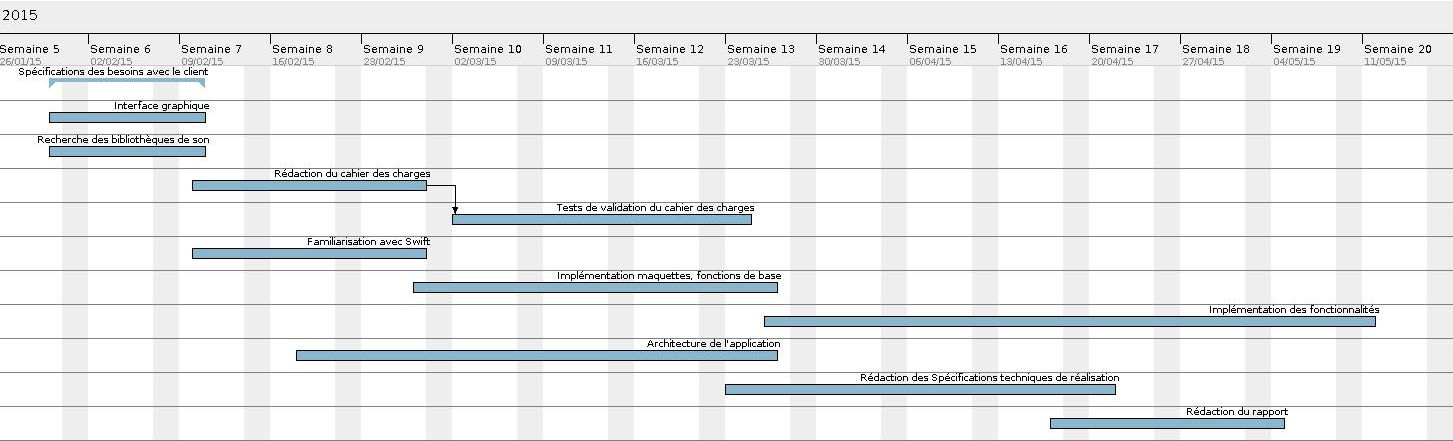
\includegraphics[width=\textwidth]{images/gantt.png}
      \caption{Notre organisation dans le temps}
\end{figure}

Durant toute la durée du projet, des réunions avec l'encadrant et le client ont été planifiées pour tester l'application et faire un bilan de so implémentation. Des comptes rendus ont été rédigés et ajoutés à l'annexe de ce rapport.

\section{Documents produits}

\noindent Les différents documents produits lors de ce projet sont :
\begin{itemize}
	\item Le cahier des charges, spécifiant tous les besoins de l'application pour le client
	\item Les Spécifications Techniques de Réalisation (STR), décrivant l'analyse de l'architecture de l'application et de son implémentation avant la phase de développement
	\item Les comptes rendus joints dans l'annexe
	\item Le présent rapport
\end{itemize}


\chapter{Conclusion}

\section{L'application iBalezator}

Durant ce projet, nous avons développé l'application iBalezator, adaptation pour terminaux \textit{iOS} du Balezator en ligne. 
Les deux modes de jeux décrits dans le cahier des charges -- manche/clavier et portée/manche -- ont été implémentés. \\
La prise en charge du son, du score, du placement des notes sur la portée, de l'enchaînement des questions, et l'interface graphique en générale
ont été implémentés dans leur intégralité et permettent aujourd'hui à l'application d'être utilisée.


Pendant toute la durée du développement, nous avons mené une réflexion sur les différentes spécificités de la musique  notamment le fonctionnement d'un manche de guitare, 
ou la représentation graphique des notes sur une portée. Cela nous a permis d'écrire des algorithmes solides qui pourraient être utilisés pour d'éventuelles améliorations
de l'application.



\section{Améliorations possibles de l'application}
Les événements réceptionnés par les vues sont directement relayés au contrôleur homonyme sans traitement.
Les contrôleurs associés à chaque vue sont présents pour masquer la partie graphique de l'application aux classes gérant la logique métier.
Pour cela, le contrôleur du manche convertit les cordonnées de tap sur le manche en Note intelligible par le reste de l'architecture.
Si l'on souhaite dans le futur changer l'image du manche ou proposer le mode gaucher, le reste de l'application n'en est pas affecté.
\newline

Il peut être utile de proposer à l'utilisateur de changer l'accordage de sa guitare.
Pour effectuer nos calculs de Note sur le manche, nous passons par un tableau qui stocke les intervalles entre les codres de la guitare.
Dans notre modèle, une note n'est qu'un couple <Frette,Corde> matérialisé par la classe Note.
Si l'on voulait changer l'accordage, il suffirait de donner un autre tableau à la classe Note pour paramétrer les fonctions de conversion.
\newline

Les vues sont calculées en proportion d'écran, la portée est dessinée à l'exécution et le manche n'est qu'une image couplée à un tableau de coordonnées pour faire corespondre un tap à une note.
Si l'on voulait adapter l'application à d'autre type de terminaux, d'autres tailles d'écran cela serait, à priori, possible sans trop de difficultés.
Les vues s'adapterons aux proportions de l'écran. 
Pour l'affichage de la portée, seul un coefficient multiplicateur est à appliquer aux coordonnées des tracés.
Enfin, pour l'affichage du manche, en fonction des dimensions de l'image utilisée et du terminal il faudra changer le tableau de coordonnées d'image des frettes et cordes.\\
\newline

Le manche de la guitare est pour le moment une image.
Il serait possible, comme pour la portée, de le dessiner au moment de l'exécution.
Un manche de guitare possède des proportions calculables.
Une formule mathématique permet d'obtenir la distance nécessaire entre chaque frette.
Cette formule est valable pour n'importe quel instrument à corde.
Ceci pourrait donc nous permettre d'afficher n'importe qu'elle manche d'instrument à corde et donc de ne pas uniquement proposer la guitare à 24 frettes.
Il faudrait cependant s'assurer que le dessin de l'image du manche n'est pas trop gourmand en ressources et n'affecte pas la fluidité de l'application.
Ceci n'a pas été le cas lorsque nous avons décidé de dessiner la portée plutôt que d'afficher une image.
\newline

La bibliothèque de son que nous utilisons est puissante, elle possède de nombreux réglages modifiables à l'exécution.
Ses nombreuses simulations d'instruments nous permettraient d'adapter le son des notes aux futurs éventuels instruments proposés par l'applcation.
On peut également prévoir une intrerface permettant à l'utilisateur de modifier ses propres réglages.
La génération de son étant encapsulée dans la classe \texttt{SoudController}, il suffirait de lui passer les paramètres utilisateurs pour qu'il puisse jouer la note en fonction.
Les paramètres de forme d'onde, de réverbération, de bruit, ... seront laissés à l'utilisateur tandis que la fréquence (qui caractérise une note) sera elle gérée par l'application. 
\newline

Notre application répond au patron de conception MVC.
Ainsi, la totalité des données pérennes de l'application sont stockées dans ces classes.
On y retrouve entre autres le score, le mode courant, la question/réponse courante, etc.
Après sérialisation de ces classes, nous pourrons les stocker dans la mémoire du terminal et les recharger au lancement.
Ces variables seront donc rechargées et l'utilisateur pourra continuer sa partie.
\newline

%armures de clé
La portée actuelle affiche une armure de clé en \textit{Do} majeur.
Il est intéressant pour les guitaristes d'être à l'aise dans toutes les tonalités.
Comme présenté dans la section \ref{portee}, la structure de la gamme majeure est stockée dans un tableau que l'on parcourt séquenciellement et cycliquement (modulos).
Pour ne pas rentrer trop dans les détails de solfège, il faut juste retenir que dans notre algorithme, s'il reste un demi-ton à consommer à la fin de la boucle, la note est diésée.
Changer la tonalité affichée sur la portée consistera simplement, non pas à partir de la case zéro du tableau mais à changer en fonction de la tonalité.
Par exemple, commencer pour \textit{Ré} majeur à l'indice 1, \textit{Fa} majeur à l'indice 3, \textit{Si} majeur à l'indice 5, etc.
Les tonalités mineures seront également gérées en ne se déplaçant non pas sur le tableau de la structure majeure mais sur celui de la structure mineure.


\chapter{Annexe}

\section{Lecture de notes sur le manche}


\bigbreak
\includegraphics[width=\textwidth]{images/neck.png}
\bigbreak

Un manche de guitare est composée de 6 cordes (représentées horizontalement sur l'image ci-dessus) et de 24 frettes (verticalement sur l'image).
La partie la plus à gauche, en jaune, s'appelle le sillet. Plus on s'éloigne du sillet et plus la note est aigüe sur la corde concernée.
Les cordes sont, de haut en bas : mi (aigu), si, sol, ré, la, mi (grave). Ce sont les notes jouées pour les cordes dites \enquote{à vide}, c'est-à-dire sans pincer aucune corde sur les cases du manche.\\

Les notes d'une gamme sont \textit{Do}, \textit{Do}\#, \textit{Ré}, \textit{Ré}\#, \textit{Mi}, \textit{Fa}, \textit{Fa}\#, \textit{Sol}, \textit{Sol}\#, \textit{La}, \textit{La}\#, \textit{Si}. Elles sont séparées par un intervalle appelé \enquote{demi-ton}. Par exemple entre \textit{Do} et \textit{Do}\#, nous avons un demi-ton.
Les frettes sont placées tous les demi-tons sur le manche de la guitare. De cette façon entre deux frettes, nous avons toujours un demi-ton. Par exemple pour la corde de \textit{Mi}, la première frette nous donne un \textit{Fa}, la deuxième un \textit{Fa}\#, la troisième un \textit{Sol}, et ainsi de suite.

Pour lire une note sur le manche de la guitare, on doit donc se placer sur la corde en question, puis l'augmenter de demi-ton en demi-ton jusqu'à arriver à la note voulue, à la frette désirée.
Par exemple, pour la corde de \textit{Mi} aigu, sur la troisième frette, on obtient un \textit{Sol} (\textit{Mi} augmenté de trois demi-tons dans la gamme).

Compte tenu de la disposition des cordes et des frettes sur une guitare, il est possible d'obtenir la même note (= la même fréquence) à plusieurs endroits différents du manche.

\newpage
\section{Lecture de notes sur la portée}

\bigbreak
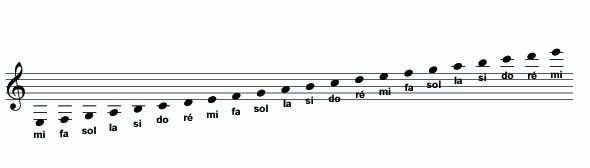
\includegraphics[width=\textwidth]{images/note_portee.jpg}
\bigbreak

Une portée est constituée de 5 lignes. 
Les notes peuvent être disposées sur une ligne ou entre deux lignes. Les notes sur la partie basse de la portée sont graves, et celles de la partie haute sont aigues. 
Lorsque les notes sont plus graves ou plus aigues que celles placées dans la portée, on trace des lignes supplémentaires. Sur l'image ci-dessus, des lignes ont été ajoutées du \textit{Mi} au \textit{Do} graves et du \textit{La} au \textit{Mi} aigus.\\
En mode portée/manche, les notes possibles affichées sur la portée seront celles ci-dessus.
La portée contient 3 otaves. \\
Les notes représentées correspondent aux notes sur le manche de la guitare jusqu'à la 12ème frette, corde 1. 
Au delà de la 12ème frette corde 1, et donc au delà du \textit{Mi} inclus, les notes sont représentées à l'octave du dessous avec une indication \texttt{8va}.

\section{Comptes rendus des réunions}
\end{document}
